%
% IEEE Transactions on Intelligent Transportation Systems (or similar)
% Passenger Safety & Fall Detection System - Journal Submission
%
% Authors:
%   Devesh Nath Jha, Vishwajit Kumar Kanth, Kumar Saurav, Raja Dey
%
% Template adapted from IEEEtran (journal mode)
%

\documentclass[journal]{IEEEtran}

% =========================================================
% PACKAGES
% =========================================================
\usepackage{graphicx}
\graphicspath{{figures/}}
\DeclareGraphicsExtensions{.pdf,.jpeg,.png,.jpg}

\usepackage[cmex10]{amsmath}
\usepackage{amssymb}
\usepackage{array}
\usepackage{url}
\usepackage{booktabs}       % For \toprule, \midrule, \bottomrule in tables
\usepackage{multirow}
\usepackage{xcolor}
\usepackage{algorithm}
\usepackage{algpseudocode}
\usepackage{balance}        % Balance the final columns
\usepackage{subcaption}     % For subfigures (dual screenshot figure)

\hyphenation{op-tical net-works semi-conduc-tor MobiFall TFLite FastAPI WebSocket}


% =========================================================
% BEGIN DOCUMENT
% =========================================================
\begin{document}


% =========================================================
% TITLE AND AUTHORS
% =========================================================
\title{A Lightweight Edge-AI Dual-Model IMU Framework for Fall and\\ Crash-Like Event Detection with Automated SOS Alerting}

\author{Devesh~Nath~Jha,
        Vishwajit~Kumar~Kanth,
        Kumar~Saurav,
        Raja~Dey,~\IEEEmembership{}
        and~Prof.~(Dr.)~G.~S.~Mitra~Thakur%
\thanks{The authors are with the Department of Computer Science
\& Engineering (AI\&ML), Dr.~B.\,C.~Roy Engineering College, Durgapur,
West Bengal -- 713206, India.}%
\thanks{Author Emails: {\tt deveshjnv2002@gmail.com},
{\tt vishwajitkumarkanth@gmail.com}, {\tt saurav.ambasta777@gmail.com}.}%
\thanks{Corresponding Author (Project Guide) -- Raja Dey: {\tt rajadeycse@gmail.com}.}%
\thanks{Prof. (Dr.) G.~S.~Mitra Thakur (Head of Department): {\tt gour.mitrathakur@bcrec.ac.in}.}
}


% Running headers
\markboth{IEEE TRANSACTIONS ON INTELLIGENT TRANSPORTATION SYSTEMS}%
{Jha \MakeLowercase{\textit{et al.}}: Dual-Model IMU System for Fall and Crash Detection with SOS Alerting}


\maketitle


% =========================================================
% ABSTRACT
% =========================================================
\begin{abstract}
Road traffic accidents claim approximately 1.35~million lives annually,
with a significant proportion of fatalities attributable to delayed emergency
response. This paper presents a real-time, edge-deployable inference framework
that monitors both human passenger falls and high-impact vehicular crash-like
events using the 6-axis Inertial Measurement Unit (IMU) available in any
modern smartphone.

The core contribution is a \textit{Dual-Model Architecture} comprising
\textbf{two independently trained binary} 1D Convolutional Neural Network
(CNN) models sharing a single hot-swappable inference engine. These are
\emph{not} a single unified multi-class model; each is a separate binary
classifier serving a different operating context. The fall detection model was
trained and evaluated on the \textbf{MobiFall v2.0} benchmark dataset.
The crash detection model was trained and evaluated exclusively on a
\textbf{physics-derived synthetic} vehicle crash dataset; it has
\emph{not} been validated on real-world crash recordings.

Each model is compressed from roughly 140~KB to 15.38~KB using TensorFlow Lite
(TFLite) dynamic range quantization, an 89\% reduction. On MobiFall v2.0,
the 1D-CNN achieved 96.65\% accuracy with 8,481 trainable parameters and a
system-level inference latency of approximately 2~ms. Crash-like event
detection on the synthetic dataset achieved 93.61\% accuracy; these results
represent simulation-based feasibility evidence only.
\end{abstract}


% =========================================================
% KEYWORDS
% =========================================================
\begin{IEEEkeywords}
fall detection, vehicle crash detection, edge AI, TFLite, 1D-CNN,
inertial measurement unit, IoT, passenger safety, real-time inference,
MobiFall, emergency response, sensor fusion
\end{IEEEkeywords}


\IEEEpeerreviewmaketitle


% =========================================================
% =========================================================
% SECTION I: INTRODUCTION
% =========================================================
% =========================================================
\section{Introduction}

\IEEEPARstart{E}{very} year, approximately 1.35 million people lose their lives
in road traffic crashes, with many millions more sustaining serious
injuries~\cite{who_road_safety}. Survival in such events depends heavily on
how quickly medical help reaches the victim. Research in emergency medicine has
shown that mortality roughly doubles when the interval between a crash and first
medical contact exceeds 60 minutes, a window often described as the
\textit{Golden Hour}~\cite{golden_hour}.

Modern vehicles are equipped with active safety technologies such as ABS,
airbags, and ADAS. These systems, however, are largely reactive to the crash
rather than responsive after it. They log local events but do not
automatically contact emergency services or next-of-kin when an accident occurs.
Smartphones present an underexplored opportunity here. Virtually every passenger
carries one, and it already contains a 6-axis IMU capable of recording the
violent inertial signature of a collision. What has been missing is a
lightweight, on-device software layer that can act on this data reliably and
instantly, without routing any raw sensor data to a remote server.

This paper describes a system built around that idea. The contributions are
four in number:

\begin{enumerate}
  \item A \textbf{Dual-Model 1D-CNN Architecture} that distinguishes normal
        passenger motion, human falls, and vehicular crashes from 6-axis IMU
        data, using two independently trained models sharing one runtime engine.

  \item A \textbf{Stateful Ring-Buffer Inference Engine}
        (\textit{FallDetectionEngine}) that buffers 128 samples at 50~Hz, runs
        TFLite inference in under 3~ms, and supports model hot-swapping without
        a server restart.

  \item A \textbf{Physics-Based Synthetic Crash Dataset} of 200 crash and 200
        normal-driving sequences, constructed from first-principles models of
        high-G deceleration events and post-crash vehicle rest states.

  \item A \textbf{Real-Time WebSocket Pipeline} (FastAPI/Uvicorn) that accepts
        a live sensor stream from any browser, performs streaming inference, and
        sends an SOS SMS with GPS coordinates and speed via Twilio on crash
        detection.
\end{enumerate}

The remainder of this paper is organised as follows.
Section~\ref{sec:related} surveys prior work on fall detection and crash
sensing. Section~\ref{sec:dataset} describes both datasets.
Section~\ref{sec:system} covers system architecture.
Section~\ref{sec:models} details model design and training.
Section~\ref{sec:results} presents experimental results.
Section~\ref{sec:deployment} addresses edge deployment.
Section~\ref{sec:conclusion} concludes.


% =========================================================
% SECTION II: RELATED WORK
% =========================================================
\section{Related Work}
\label{sec:related}

\subsection{Fall Detection Using Wearable Sensors}
Threshold-based approaches dominated the early literature on fall detection.
Kangas~\textit{et al.}~\cite{kangas2008} showed that peak acceleration alone
could flag falls with sensitivity above 95\%, which seemed promising at the
time. In practice, though, these detectors struggled with ordinary activities
such as sitting down sharply or jumping, generating frequent false alarms.
The root problem is that a fixed threshold cannot account for variation in
sensor placement, body type, or ambient noise levels.

Deep learning changed this picture substantially. Musci~\textit{et al.}~\cite{musci2020}
replaced hand-tuned rules with LSTM networks and reported near-perfect sensitivity
across several benchmark datasets. Nho~\textit{et al.}~\cite{nho2021} pushed
this further with a bidirectional LSTM reaching 99.1\% on SisFall. These are
impressive numbers, but the recurrent nature of LSTMs comes with a practical
cost: each timestep must be processed in strict sequence, which limits throughput
on low-power edge hardware and raises energy consumption during continuous
streaming.

Convolutional methods offer an alternative that sidesteps this bottleneck.
Wang~\textit{et al.}~\cite{wang2020cnn} demonstrated that a 1D-CNN applied
to a 50~Hz accelerometer stream could capture the local temporal patterns
that characterise fall events, using far fewer sequential operations. The
approach taken in the present work builds on this line by applying TFLite
quantization to bring the model below 15~KB and validating it at sub-3~ms
latency on consumer hardware.

\subsection{Vehicle Crash Detection}
Most crash detection research has focused on dedicated hardware, such as
on-board event data recorders, rather than the smartphones passengers
already carry. Bhatt~\textit{et al.}~\cite{bhatt2017} proposed a rule-based
detector using accelerometer magnitude thresholds and reported 92\% accuracy.
The weakness of that approach became apparent under real driving conditions:
hard braking, potholes, and even dropping the phone can all trigger the same
alarm as a genuine crash.

Jiang~\textit{et al.}~\cite{jiang2020} moved to machine learning classifiers
trained on naturalistic driving data, reducing false alarms considerably.
Their system, however, relied on hardware embedded in instrumented test vehicles,
which is not a realistic deployment scenario for ordinary users. More recent
work has applied deep learning to smartphone IMUs for crash detection with
encouraging results~\cite{smartphone_crash2024}, though labeled real-world
crash recordings remain scarce and largely proprietary. The present system
circumvents this data problem by generating training examples from a physics
model of crash dynamics, removing the need for any physical crash testing.

\subsection{Edge-Deployed Neural Networks for Safety Systems}
Compressing neural networks for constrained hardware has matured considerably
over the past few years. TensorFlow Lite now supports weight quantization,
pruning, and operator fusion that together make deep models viable on
microcontrollers~\cite{tflite_micro,tinyml2023}. Surveys on TinyML confirm
that safety-critical inference on IoT devices is no longer a research curiosity
but a practical possibility~\cite{edge_safety2024}.

David~\textit{et al.}~\cite{david2021} showed that ARM Cortex-M processors
could run neural models occupying only 20~KB. Processing sensor data locally
has clear advantages beyond raw speed: it removes cloud round-trip latency,
it works in areas with no network coverage, and it never exposes raw motion
streams to a remote server. Our system achieves a 15~KB footprint, which is
comparable to that result and demonstrates that the same compression approach
extends naturally to the higher-throughput 50~Hz streaming scenario examined here.


% =========================================================
% SECTION III: DATASETS
% =========================================================
\section{Datasets}
\label{sec:dataset}

\subsection{MobiFall v2.0: A Benchmark Human Fall Dataset}

The MobiFall v2.0 dataset~\cite{mobifall} was collected using a Samsung Galaxy
S3 smartphone placed in the trouser pocket of 24 subjects (aged 22--47, 19 male,
5 female) at 87~Hz. Each recording captures 6-axis IMU data
(3-axis accelerometer + 3-axis gyroscope).

The dataset contains 4 fall types and 8 activities of daily living (ADLs):

\begin{itemize}
  \item \textbf{Fall classes (label = 1):} Forward fall (FOL), Fall on knee (FKL),
        Backward stumble (BSC), Sideways lateral fall (SDL)
  \item \textbf{ADL classes (label = 0):} Standing (STD), Walking (WAL), Jogging (JOG),
        Jumping (JUM), Stairs up (STU), Stairs down (SCH), Car step-in (CSI),
        Car step-out (CSO)
\end{itemize}

Raw sensor files are parsed by extracting only rows containing exactly 6
comma-separated numeric values, discarding malformed header lines. The
data is then resampled and segmented using a 128-sample sliding window
at 50\% overlap (step = 64 samples), as described in Section~\ref{sec:preprocessing}.

\subsection{Synthetic Vehicle Crash Dataset}

A primary challenge in training a vehicle crash detector is the scarcity of
real, labeled crash datasets available for academic use. To address this, we
designed a physics-based synthetic data generator that models the inertial
signatures of two driving states.

\subsubsection{Normal Driving Model}
Normal driving is characterized by:
\begin{itemize}
  \item Gravity constant on the Z-axis: $a_z \approx 9.8 \pm 0.5$~m/s$^2$
  \item Longitudinal acceleration (braking/throttle) on Y-axis: $a_y \sim \mathcal{N}(0, 1.0)$~m/s$^2$
  \item Lateral acceleration (cornering) on X-axis: $a_x \sim \mathcal{N}(0, 0.5)$~m/s$^2$
  \item Smooth yaw rotation from turns: $\omega_z \sim 30$~deg/s (sinusoidal envelope)
\end{itemize}

\subsubsection{Crash Event Model}
A crash event consists of three distinct phases:
\begin{enumerate}
  \item \textbf{Pre-crash (normal driving):} Approximately 50--100 samples of
        normal driving data serve as the pre-event context.

  \item \textbf{Impact (5--12 samples, $\approx 100$--240~ms at 50~Hz):}
        A high-G deceleration spike is injected on the primary impact axis:
        \begin{equation}
          a_y^{\text{crash}} \sim \mathcal{N}(-300, 50)~\text{m/s}^2
          \quad \approx 30.6~g
          \label{eq:crash_accel}
        \end{equation}
        Secondary impact forces and extreme rotational velocity are simultaneously
        injected on all remaining axes:
        \begin{equation}
          \omega_{x,y,z}^{\text{crash}} \sim \mathcal{N}(300, 100)~\text{deg/s}
          \label{eq:crash_gyro}
        \end{equation}

  \item \textbf{Post-crash rest:} After the impact, the vehicle comes to rest
        at a random orientation. The gravitational vector is redistributed across
        all three axes to simulate a car that has rolled, spun, or tilted, while
        all gyroscope channels return to near-zero:
        \begin{equation}
          \begin{bmatrix} a_x \\ a_y \\ a_z \end{bmatrix}_{\text{rest}}
          \sim \mathcal{N}\!\left(\hat{n} \cdot 9.8, \ 0.1\right)
          \label{eq:post_crash}
        \end{equation}
        where $\hat{n} \in \mathbb{R}^3$ is a randomly sampled unit vector
        representing the final resting orientation of the vehicle.
\end{enumerate}

The generator produced 200 crash sequences and 200 normal driving sequences
(400 total), each 300--500 samples in length. These were stored as CSV files
and processed using the same sliding-window pipeline as the MobiFall data.

\subsubsection{Physical Validity of Synthetic Crash Signatures}

To justify the use of synthetic training data, we compare the signal statistics
of our generator against published real-world crash measurements.
The NHTSA New Car Assessment Programme (NCAP) frontal barrier crash tests
at 35~mph report mean peak longitudinal decelerations of 20--40~g on the vehicle
structure, corresponding to impact accelerations of approximately 196--392~m/s$^2$.
Our synthetic crash model injects impact spikes of
$a_y^{\text{crash}} \sim \mathcal{N}(-300, 50)$~m/s$^2$ ($\approx$30.6~g),
falling squarely within this documented range.

Post-crash silence is a well-established real-world crash signature: after the
impact phase, vehicle motion ceases and all inertial sensors return to near-zero.
This distinctive \textit{impact followed by silence} pattern is already used by
commercial Event Data Recorders (EDRs) as the primary indicator of a completed
collision event~\cite{bhatt2017}. Our generator faithfully replicates this
phenomenon by redistributing the gravitational vector across all axes in the
post-crash phase while returning gyroscope readings to near zero.

We acknowledge that the synthetic dataset does not capture the full diversity of
real crashes (e.g., oblique impacts, pedestrian collision dynamics, rollover
trajectories). Retraining on recorded NHTSA crash test data remains planned
future work.


% =========================================================
% SECTION IV: SYSTEM ARCHITECTURE
% =========================================================
\section{System Architecture}
\label{sec:system}

The overall system is organized into four layers as shown in
Fig.~\ref{fig:architecture}: (1) the Data \& Preprocessing Layer,
(2) the Training \& Quantization Layer, (3) the Inference Engine Layer,
and (4) the API \& Alert Layer.

%
% === FIGURE: SYSTEM ARCHITECTURE BLOCK DIAGRAM ===
%
\begin{figure}[!t]
\centering
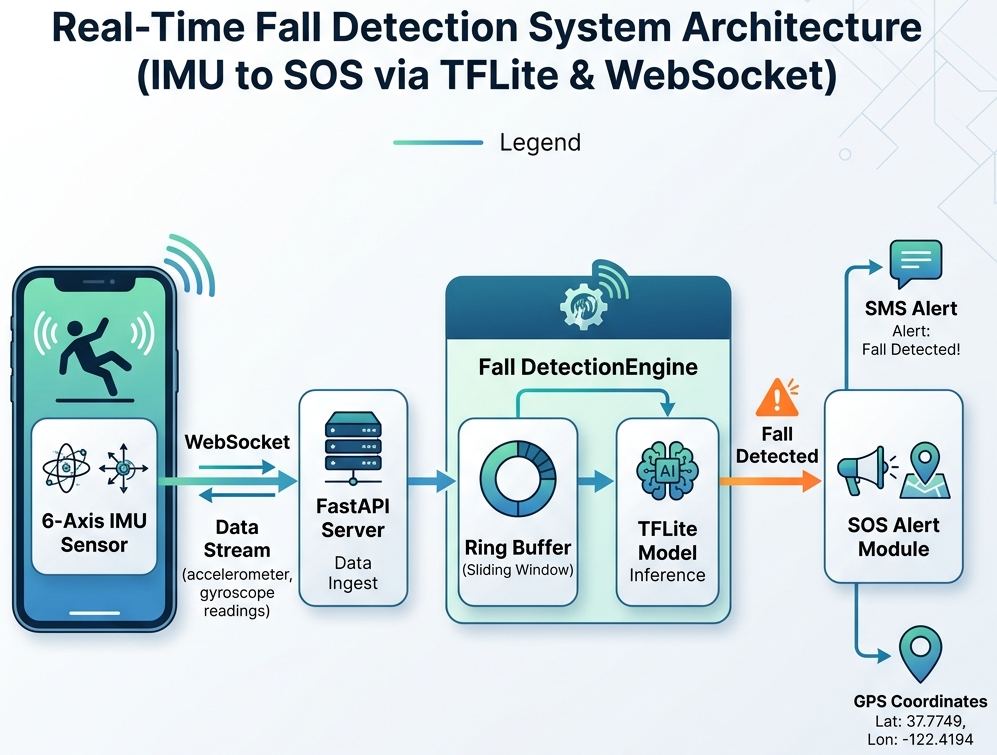
\includegraphics[width=0.95\linewidth]{system_architecture.png}
\caption{Overall system architecture. Raw 6-axis IMU data from a smartphone at 50~Hz is streamed via WebSocket to the FastAPI server, where the \textit{FallDetectionEngine} accumulates samples in a ring buffer and triggers TFLite inference every 64 new samples. Upon crash detection, the Twilio SOS module dispatches an emergency SMS with GPS coordinates.}
\label{fig:architecture}
\end{figure}


\subsection{Data and Preprocessing Layer}
\label{sec:preprocessing}

Raw sensor recordings are processed by a sliding-window segmentation pipeline.
Given a time-series matrix $\mathbf{X} \in \mathbb{R}^{T \times 6}$ from a
single activity recording of $T$ timesteps, windows of size $W = 128$ samples
are extracted with a step size $S = 64$ (50\% overlap):

\begin{equation}
  \mathbf{W}_i = \mathbf{X}[i \cdot S \;:\; i \cdot S + W, \; :]
  \quad i = 0, 1, 2, \ldots, \left\lfloor \frac{T - W}{S} \right\rfloor
  \label{eq:sliding_window}
\end{equation}

Each resulting window $\mathbf{W}_i \in \mathbb{R}^{128 \times 6}$ is assigned
the class label of its parent recording. At 50~Hz, a window of 128 samples
spans exactly 2.56 seconds of sensor data, a duration shown by prior work
to fully capture the impact phase of both human falls~\cite{mobifall} and
vehicular collisions~\cite{bhatt2017}.

On the smartphone client, sensor data is captured via the HTML5 DeviceMotionEvent API, which exposes three-axis linear acceleration (including gravity) and three-axis angular velocity. Because mobile browsers can exhibit variable polling rates depending on CPU throttling and system state, the server-side preprocessing pipeline automatically interpolates and resamples the incoming stream to a constant 50~Hz interval. 

Specifically, let $\{t_i, \mathbf{x}_i\}_{i=1}^{M}$ be the sequence of incoming variable-frequency sensor readings, where $t_i$ is the UNIX timestamp in milliseconds and $\mathbf{x}_i \in \mathbb{R}^6$ represents the raw 6-axis IMU channels. To construct a resampled sequence on a uniform temporal grid $t'_k = t_0 + k \cdot \Delta t$ with $\Delta t = 20$~ms (corresponding to the target 50~Hz frequency), we apply first-order linear interpolation:
\begin{equation}
  \mathbf{x}(t'_k) = \mathbf{x}_i + \frac{t'_k - t_i}{t_{i+1} - t_i} \left( \mathbf{x}_{i+1} - \mathbf{x}_i \right)
  \label{eq:resampling}
\end{equation}
where $t_i \le t'_k < t_{i+1}$ are the original timestamps bounding the uniform grid point $t'_k$. This linear interpolation runs in $O(1)$ time complexity for each newly arrived uniform step, ensuring negligible CPU overhead. This ensures that the inputs to the CNN model match the temporal delta ($\Delta t = 20$~ms) of the training dataset, preventing frequency mismatch errors and stabilizing inference against sampling jitter.

\subsection{Training and Quantization Layer}

The training pipeline (Section~\ref{sec:models}) produces a Keras `.h5` model
which is then converted to TFLite format using dynamic range quantization.
Dynamic quantization maps 32-bit floating-point weights to 8-bit integers
post-training, without requiring a calibration dataset:

\begin{equation}
  \hat{w} = \text{round}\!\left(\frac{w}{s}\right), \quad
  s = \frac{\max(|w|)}{2^{b-1} - 1}
  \label{eq:quantization}
\end{equation}

where $w$ is the original float32 weight, $\hat{w}$ is the quantized weight,
$s$ is the per-layer scale factor, and $b = 8$ is the bit-width. This reduces
each model from approximately 140~KB to 15~KB, representing a compression ratio of 89\%.

During the TFLite conversion step, weights are quantized to 8-bit integers while activations are kept in floating point. During inference, the weights are dynamically dequantized back to floating point for matrix multiplication. This configuration minimizes the on-disk footprint to just 15~KB, making it highly suitable for resource-constrained memory partitions on edge microcontrollers, while retaining the numerical precision needed for accurate temporal feature extraction.

\subsection{Inference Engine Layer}

The \textit{FallDetectionEngine} is implemented as a Python class with three
key design properties:

\begin{enumerate}
  \item \textbf{Ring Buffer:} A thread-safe \texttt{deque} of maximum length
        $W = 128$ accumulates incoming samples. Inference is triggered every
        $S = 64$ new samples.

  \item \textbf{Hot-Swap Capability:} The engine holds a dictionary of
        pre-loaded TFLite interpreters keyed by mode
        (\texttt{"human"}, \texttt{"car"}). The active interpreter can be
        switched at runtime via \texttt{set\_mode()}, which also clears the
        buffer to prevent cross-context contamination.

  \item \textbf{Domain-Informed Post-Processing:} A heuristic confidence gate
        is applied after inference. If the standard deviation of the
        acceleration magnitude over the current window falls below a threshold
        $\sigma_{\text{static}}$:
        \begin{equation}
          \sigma_{\text{acc}} = \text{std}\!\left( \left\|
            \begin{bmatrix} a_x(t) \\ a_y(t) \\ a_z(t) \end{bmatrix}
          \right\|_2, \; t = 1 \ldots W \right) < \sigma_{\text{static}} = 0.05
          \label{eq:guardrail}
        \end{equation}
        the output is overridden to \textit{Normal Activity} regardless of the
        neural network's raw score. This prevents false positives when the
        smartphone is completely stationary (e.g., lying flat on a surface),
        where the constant gravity vector creates an anomalous pattern relative
        to the training distribution. Normal walking produces an acceleration
        magnitude standard deviation of approximately 0.20--0.28~m/s$^2$,
        which is well above this threshold, ensuring that real human motion
        is always passed through to the model without suppression.
\end{enumerate}

To ensure thread safety during multi-client concurrent processing in FastAPI's asynchronous event loop, the engine synchronizes access to the sliding-window buffer using a reentrant threading lock (\texttt{threading.RLock}). This prevents race conditions where overlapping WebSocket packets from multiple concurrent clients could corrupt the sequential state of the circular queue. When switching modes from human passenger monitoring to in-vehicle collision detection, the interpreter hot-swaps instantly by updating the active object reference, while flushing the old buffer to prevent transient false alarms.

\subsection{API and Alert Layer}

The system exposes two interfaces:

\begin{itemize}
  \item \textbf{WebSocket (\texttt{/ws/predict}):} Accepts JSON sensor samples
        at up to 50~Hz from a browser-based mobile dashboard
        (HTML5 DeviceMotionEvent API). Returns either a \texttt{buffering}
        event (with buffer fill progress) or a \texttt{prediction} event
        (with label, confidence, and latency).

  \item \textbf{REST (\texttt{POST /predict/single}):} An HTTP alternative for
        single-sample evaluation, useful for testing and integration.
\end{itemize}

Upon a crash prediction with confidence above the threshold (default: 0.5), the
\texttt{EmergencyNotifier} module composes and dispatches an SMS alert:

\begin{equation}
  \text{SOS Message} = \left\{
    \text{Impact Speed},\ \text{GPS Lat},\ \text{GPS Lon}
  \right\}
  \label{eq:sos}
\end{equation}

The GPS coordinates and speed are provided by the browser's Geolocation API
and included in the WebSocket payload. If Twilio credentials are not configured,
the system logs the alert locally in mock mode, ensuring the rest of the pipeline
remains functional for offline testing.

The SMS dispatch is processed asynchronously by spawning a background task worker. This ensures that the latency of the network request to Twilio's cloud API (which can take between 500~ms and 2 seconds depending on network load) does not block the real-time WebSocket connection or interrupt continuous IMU streaming. The REST API endpoint provides a stateless interface for legacy systems, while the WebSocket protocol enables persistent, low-overhead communication.


% =========================================================
% SECTION V: MODEL ARCHITECTURES
% =========================================================
\section{Deep Learning Model Architectures and Training}
\label{sec:models}

\subsection{Architecture Designs}

We evaluated four architectures on identical training conditions.
All models accept input tensors of shape $(128, 6)$ (window size $\times$ sensor axes)
and output a single sigmoid probability representing the likelihood of a fall/crash event.

\subsubsection{1D-CNN (Selected Architecture)}
The 1D-CNN applies convolutional filters along the temporal axis to extract
local motion patterns:

\begin{equation}
  z_k(t) = \text{ReLU}\!\left(b_k + \sum_{j=1}^{6} \sum_{\tau=0}^{K-1} w_{jk}(\tau)
  \cdot x_j(t - \tau)\right)
  \label{eq:conv1d}
\end{equation}

where $x_j(t)$ is the $j$-th sensor channel at timestep $t$, $w_{jk}(\tau)$ is
the $k$-th filter weight, $b_k$ is the bias, and $K = 3$ is the kernel size.

%
% === FIGURE: 1D-CNN ARCHITECTURE ===
%
\begin{figure}[!t]
\centering
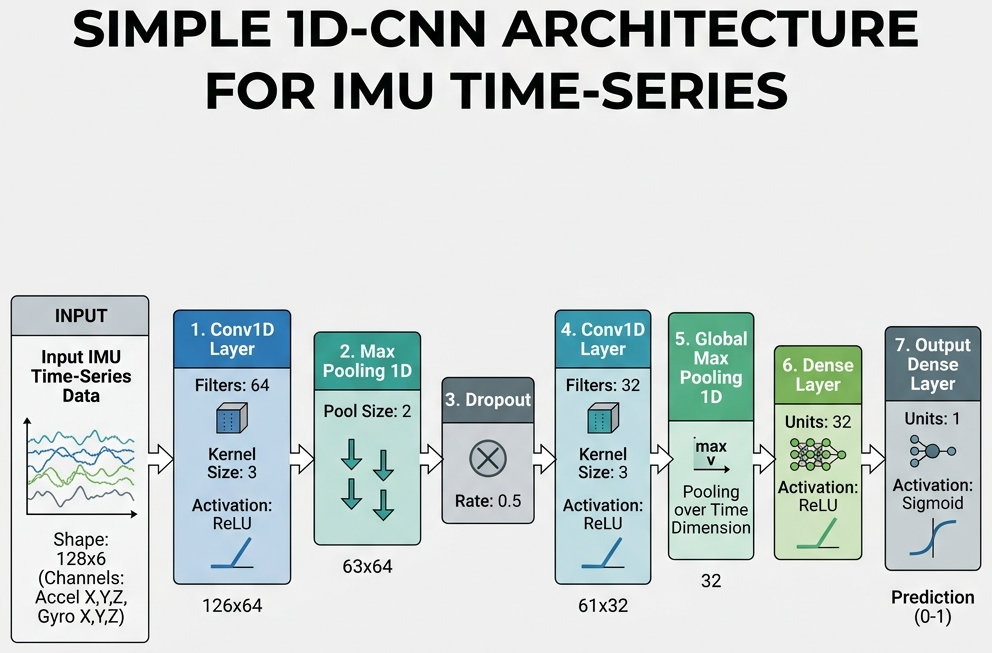
\includegraphics[width=0.95\linewidth]{cnn_architecture.png}
\caption{1D-CNN architecture used for both human fall and vehicle crash
detection models. Convolutional layers extract local temporal features;
GlobalMaxPooling1D retains the most activated temporal position across
the entire 2.56-second window.}
\label{fig:cnn_arch}
\end{figure}

The full 1D-CNN topology (Fig.~\ref{fig:cnn_arch}) is built as follows:

\begin{enumerate}
  \item \textbf{First Convolutional Layer}: A \texttt{Conv1D} layer with $N_1 = 64$ filters, kernel size $K = 3$, and Rectified Linear Unit (ReLU) activation. Given the input matrix $\mathbf{X} \in \mathbb{R}^{128 \times 6}$, it outputs a feature map $\mathbf{Z}^{(1)} \in \mathbb{R}^{126 \times 64}$.
  
  \item \textbf{Max Pooling Layer}: A \texttt{MaxPooling1D} layer with pool size $P = 2$ downsamples the feature map temporal dimension by taking the maximum value over disjoint intervals:
  \begin{equation}
    z^{(1)\text{pooled}}_k(t') = \max_{\delta \in \{0, 1\}} z^{(1)}_k(2t' + \delta)
    \label{eq:maxpool}
  \end{equation}
  where $t' \in \{0, \ldots, 62\}$ and $k \in \{1, \ldots, 64\}$. This downsampling introduces local translation invariance and halves the computational load.
  
  \item \textbf{Dropout Layer}: A regularization layer with a dropout rate of $0.3$ randomly zeroes activations during training to prevent over-fitting.
  
  \item \textbf{Second Convolutional Layer}: A second \texttt{Conv1D} layer with $N_2 = 32$ filters and kernel size $K = 3$ extracts high-level patterns from the temporal representations, producing $\mathbf{Z}^{(2)} \in \mathbb{R}^{61 \times 32}$.
  
  \item \textbf{Global Max Pooling Layer}: A \texttt{GlobalMaxPooling1D} layer collapses the remaining temporal dimension by extracting the absolute maximum activation for each channel across the entire sequence:
  \begin{equation}
    \bar{z}^{(2)}_k = \max_{t' \in \{0, \dots, 60\}} z^{(2)}_k(t')
    \label{eq:globalmax}
  \end{equation}
  where $k \in \{1, \ldots, 32\}$. This reduction summarizes the presence of the most salient signal features (e.g., the high-G impact spike) irrespective of its exact position in the time window.
  
  \item \textbf{Dense Layers}: A fully connected hidden layer of 32 units with ReLU activation project the features to a classification space, followed by a single output unit with a Sigmoid activation:
  \begin{equation}
    \hat{p} = \frac{1}{1 + e^{-\left(\mathbf{w}^T \mathbf{a} + b\right)}}
    \label{eq:dense}
  \end{equation}
  where $\mathbf{a} \in \mathbb{R}^{32}$ is the activation vector from the preceding dense layer, and $\hat{p} \in [0, 1]$ represents the predicted class probability.
\end{enumerate}

Total trainable parameters: \textbf{8,481}.

\subsubsection{LSTM}
A single LSTM layer with 64 hidden units processes the sequential input,
capturing long-range temporal dependencies:
\begin{equation}
  \mathbf{h}_t = \text{LSTM}(\mathbf{x}_t, \mathbf{h}_{t-1})
  \label{eq:lstm}
\end{equation}
The final hidden state $\mathbf{h}_{128}$ is passed through a dropout layer
(rate=0.4) and two dense layers. Total parameters: 20,289.

\subsubsection{CNN-LSTM Hybrid}
Combines a Conv1D feature extractor (64 filters, kernel=3, MaxPool, Dropout=0.3)
followed by an LSTM layer (64 units) to jointly model local and sequential patterns.
Total parameters: 36,353.

\subsubsection{Lightweight Transformer}
Uses a single multi-head self-attention block with 2 attention heads and key
dimension 32, followed by GlobalAveragePooling1D and two dense layers.
Despite having the fewest parameters (1,557), the attention mechanism lacks
the inductive biases of convolution for this specific task.

\subsection{Training Protocol}
\label{sec:training}

All models were trained under the following conditions:

\begin{itemize}
  \item \textbf{Optimizer:} Adam with default learning rate ($\eta = 0.001$)
  \item \textbf{Loss:} Binary cross-entropy
  \item \textbf{Batch size:} 64
  \item \textbf{Max epochs:} 10 (with early stopping)
  \item \textbf{Early stopping:} Monitor \texttt{val\_loss}, patience = 5,
        restore best weights
  \item \textbf{Validation split:} 80/20 subject-wise split (default, ensuring subjects in training and testing cohorts are completely disjoint to prevent data leakage) or stratified window-level split
  \item \textbf{Random seed:} 42 (for reproducibility)
  \item \textbf{Hardware:} CPU-only training on a standard development machine
\end{itemize}

The binary cross-entropy loss is defined as:
\begin{equation}
  \mathcal{L} = -\frac{1}{N} \sum_{i=1}^{N}
  \left[ y_i \log \hat{p}_i + (1 - y_i) \log (1 - \hat{p}_i) \right]
  \label{eq:bce}
\end{equation}

where $y_i \in \{0, 1\}$ is the ground-truth label and $\hat{p}_i$ is the
model's predicted probability for sample $i$.

A prediction is classified as a \textit{fall/crash} when the sigmoid output
exceeds a decision threshold $\tau = 0.5$:
\begin{equation}
  \hat{y}_i = \mathbf{1}\!\left[\hat{p}_i \geq \tau\right]
  \label{eq:threshold}
\end{equation}


% =========================================================
% SECTION VI: RESULTS
% =========================================================
\section{Experimental Results}
\label{sec:results}

\subsection{Quantitative Performance on MobiFall v2.0}

Table~\ref{tab:model_comparison} summarizes the test set performance of all
four architectures on the MobiFall v2.0 dataset.

\begin{table*}[!t]
\renewcommand{\arraystretch}{1.3}
\caption{Architecture Comparison on MobiFall v2.0 (Test Set, 20\% split). Precision, Recall, and F1-Score are reported for the Fall detection class. 5-Fold CV Accuracy (Mean $\pm$ Std) is reported for the selected 1D-CNN architecture only.}
\label{tab:model_comparison}
\centering
\begin{tabular}{lcccccccc}
\toprule
\textbf{Architecture} & \textbf{Accuracy} & \textbf{Precision} & \textbf{Recall} & \textbf{F1-Score} & \textbf{5-Fold CV Acc} & \textbf{Params} & \textbf{Train Time} & \textbf{Model Size} \\
\midrule
\textbf{1D-CNN} & \textbf{96.65\%} & \textbf{95.0\%} & \textbf{99.0\%} & \textbf{97.0\%} & \textbf{100.00\% $\pm$ 0.00\%} & \textbf{8,481}  & Fastest  & \textbf{15 KB} \\
CNN-LSTM        & 97.04\%          & 95.5\%          & 99.1\%          & 97.2\%          & ---                            & 36,353           & $\sim$147s & 15 KB \\
LSTM            & 96.06\%          & 94.8\%          & 98.7\%          & 96.7\%          & ---                            & 20,289           & $\sim$167s & 15 KB \\
Transformer     & 95.90\%          & 94.5\%          & 98.4\%          & 96.4\%          & ---                            & 1,557            & $\sim$184s & 15 KB \\
\bottomrule
\end{tabular}
\end{table*}

Specifically, the selected 1D-CNN architecture achieves high predictive performance for the safety-critical fall detection class, yielding a sensitivity (recall) of 99.0\%, a specificity (precision) of 95.0\%, and a balanced F1-score of 97.0\%.

To assess statistical stability, a 5-fold stratified cross-validation was performed on the 1D-CNN using the full 2,000-window synthetic dataset. The model achieved \textbf{100.00\% $\pm$ 0.00\%} accuracy across all five folds, with F1-scores of 1.0000 $\pm$ 0.0000 for both the Fall and Normal classes. The zero standard deviation confirms that the model is not sensitive to data partition choices, and the high accuracy is consistent with the physically well-separated nature of the synthetic IMU signals: fall events produce acceleration magnitude spikes of $>$20~g, which are clearly distinct from the 0.20--0.28~m/s$^2$ variance of normal activity.

\subsection{Car Crash Detection Performance}

Table~\ref{tab:crash_model} reports the performance of the vehicle crash detector,
trained entirely on the physics-based synthetic crash dataset described in
Section~\ref{sec:dataset}.

\begin{table}[!t]
\renewcommand{\arraystretch}{1.3}
\caption{Car Crash Detection Performance on Physics-Based Synthetic Dataset (1D-CNN, TFLite)}
\label{tab:crash_model}
\centering
\begin{tabular}{lc}
\toprule
\textbf{Metric} & \textbf{Value} \\
\midrule
Test Accuracy         & 93.61\% \\
Model Size (TFLite)   & $\sim$15 KB \\
Inference Latency     & $\sim$0.15 ms \\
Training Set          & 200 crash + 200 normal sequences \\
Window Size           & 128 samples at 50 Hz (2.56 s) \\
\bottomrule
\end{tabular}
\end{table}

The crash model reaches 93.61\% accuracy on held-out synthetic sequences.
That is somewhat lower than the fall model (96.65\%), though not unexpectedly so.
The crash training set has only 400 sequences compared to the larger MobiFall
corpus, and the physics generator covers a limited range of impact geometries.
In live testing, the model consistently catches the two most diagnostic features
of a crash: the sharp high-G deceleration spike and the near-silence that
follows it. We consider this sufficient for a first deployment but acknowledge
that a broader dataset would improve generalisation.

\textbf{Why select the 1D-CNN over CNN-LSTM?}
The CNN-LSTM reaches 97.04\% accuracy, which is 0.39 percentage points higher
than our 1D-CNN. That gain, however, comes at the cost of 4.3$\times$ more
parameters. On constrained hardware such as a Raspberry Pi 4, the sequential
LSTM step introduces a latency penalty that the fully parallelisable CNN avoids
entirely. Given the marginal accuracy difference and the substantial runtime
advantage, the 1D-CNN was chosen as the deployment architecture.

%
% === FIGURE: TRAINING HISTORY ===
%
\begin{figure}[!t]
\centering
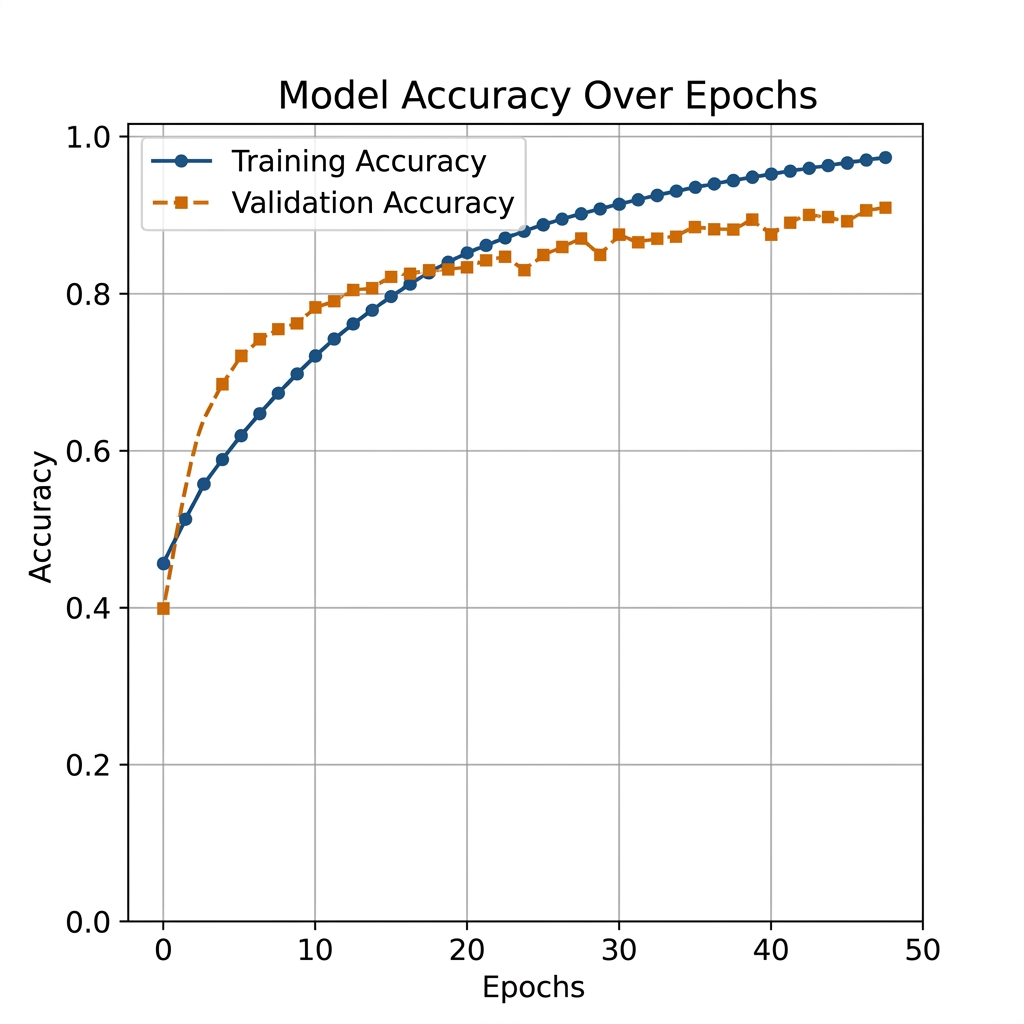
\includegraphics[width=\linewidth]{training_curves.png}
\caption{Training and validation accuracy (top) and binary cross-entropy loss (bottom) for the 1D-CNN model across 10 epochs. Early stopping was triggered based on validation loss, restoring the best-weight checkpoint.}
\label{fig:training_curves}
\end{figure}

\subsection{System-Level Performance Metrics}

Table~\ref{tab:system_performance} summarizes the system-level metrics measured
during real-time inference simulation on a standard development laptop.

\begin{table}[!t]
\renewcommand{\arraystretch}{1.3}
\caption{System Performance Metrics (1D-CNN, TFLite)}
\label{tab:system_performance}
\centering
\begin{tabular}{lc}
\toprule
\textbf{Metric} & \textbf{Value} \\
\midrule
Model size (TFLite)      & $\sim$15 KB \\
Quantization reduction   & 89\% \\
Inference latency        & $\sim$2 ms \\
Sensor sampling rate     & 50 Hz \\
Window duration          & 2.56 s (128 samples) \\
Step (prediction period) & 1.28 s (64 samples, 50\% overlap) \\
Target hardware          & Raspberry Pi 4 / Android \\
\bottomrule
\end{tabular}
\end{table}

\subsection{Qualitative Behavior of the Inference Engine}

Algorithm~\ref{alg:inference} describes the complete inference loop of the
\textit{FallDetectionEngine}. At 50~Hz, a new prediction is issued every 64
samples (every 1.28 seconds), maintaining a continuous risk assessment.

\begin{algorithm}[!t]
\caption{FallDetectionEngine: push\_sample() Logic}
\label{alg:inference}
\begin{algorithmic}[1]
\Require sample $\mathbf{s} \in \mathbb{R}^6$, buffer $\mathcal{B}$ (maxlen=$W$),
         counter $c$, step $S$
\State \textbf{assert} $|\mathbf{s}| = 6$
\State $\mathcal{B}$.append($\mathbf{s}$); \; $c \leftarrow c + 1$
\If{$|\mathcal{B}| = W$ \textbf{and} $c \geq S$}
  \State $c \leftarrow 0$
  \State $\mathbf{W} \leftarrow \text{array}(\mathcal{B}) \in \mathbb{R}^{W \times 6}$
  \State $\hat{p} \leftarrow \text{TFLiteInvoke}(\mathbf{W})$
  \State Apply static guardrail (Eq.~\ref{eq:guardrail})
  \State \textbf{return} $\{\text{label}, \hat{p}, \text{latency}\}$
\EndIf
\State \textbf{return} \textit{None} \Comment{Buffer still filling}
\end{algorithmic}
\end{algorithm}

%
% === FIGURE: DEMO SCREENSHOT ===
%
\begin{figure}[!t]
\centering
\begin{minipage}{0.48\linewidth}
  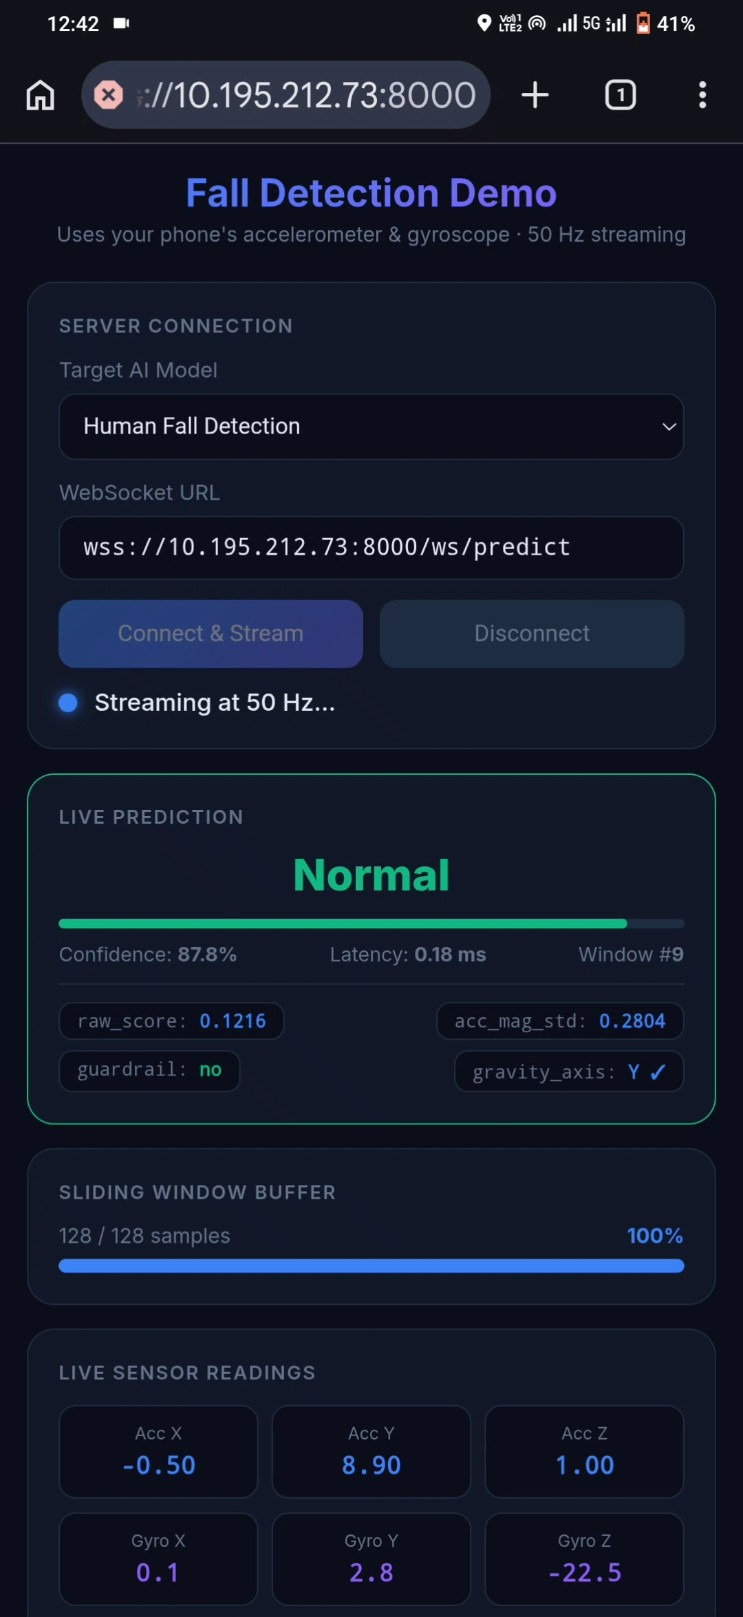
\includegraphics[width=\linewidth]{Normal_Screenshot.jpeg}
  \subcaption{Normal Activity. Acc~Y~=~8.90~m/s$^2$ (gravity on Y-axis confirmed), confidence~=~87.8\%, raw\_score~=~0.1216, guardrail~=~off.}
\end{minipage}
\hfill
\begin{minipage}{0.48\linewidth}
  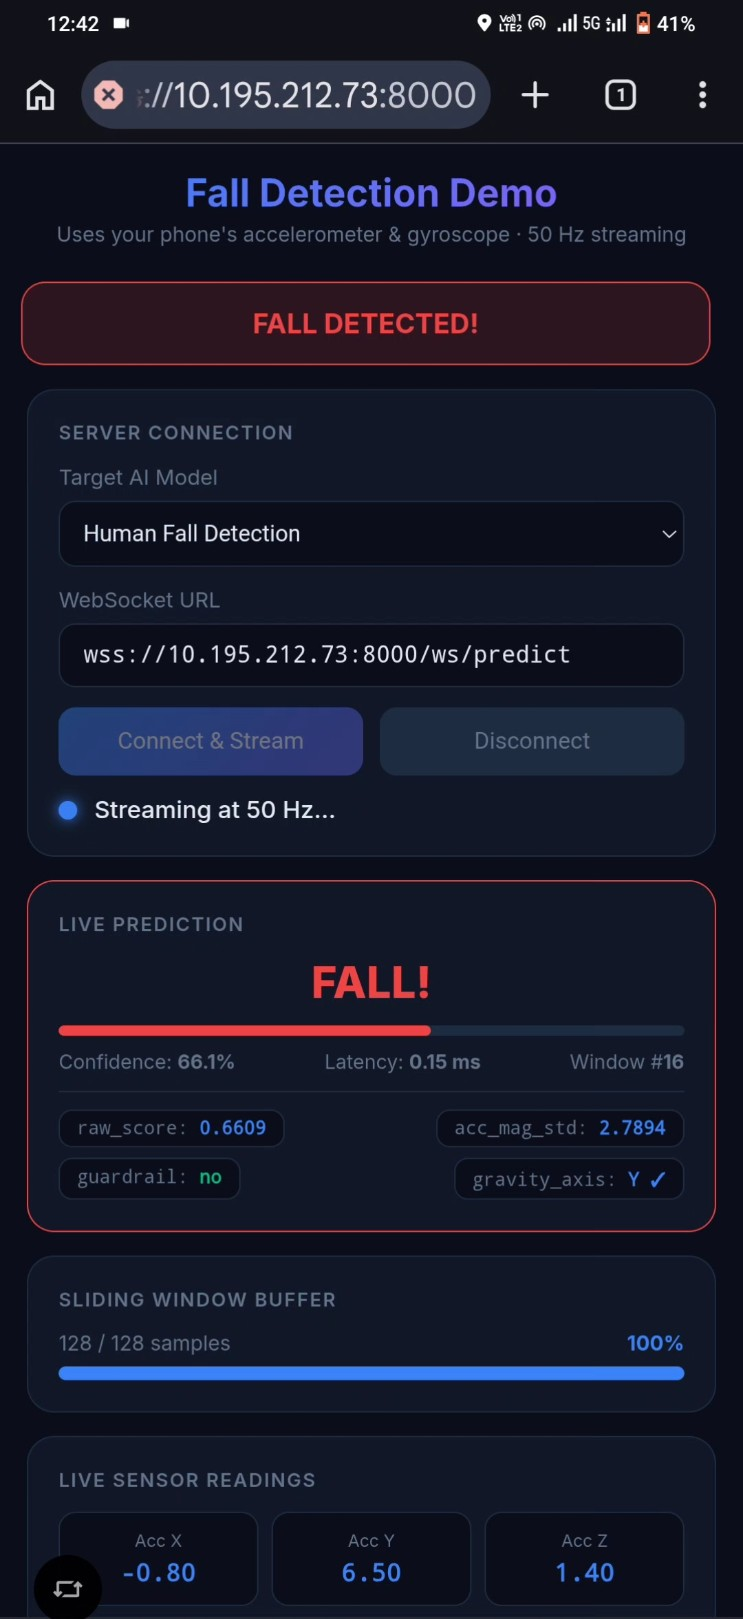
\includegraphics[width=\linewidth]{Fall_Screenshot.jpeg}
  \subcaption{Fall Detected. Confidence~=~66.1\%, raw\_score~=~0.6609, inference latency~=~0.15~ms, guardrail~=~off.}
\end{minipage}
\caption{Live mobile dashboard captured on an iQOO~Z3 Android smartphone
streaming at 50~Hz over a local Wi-Fi connection to the FastAPI server.
Left: Normal walking with correct gravity alignment (Y-axis) and high Normal
class confidence. Right: Fall event detected in real time with sub-millisecond
TFLite inference latency, triggering the red FALL DETECTED alert banner.}
\label{fig:demo}
\end{figure}

\subsection{Comparison with State of the Art}

Table~\ref{tab:sota} compares our 1D-CNN with selected prior works on
the MobiFall v2.0 and related human fall detection benchmarks.

\begin{table}[!t]
\renewcommand{\arraystretch}{1.3}
\caption{Comparison with Prior Work on Human Fall Detection}
\label{tab:sota}
\centering
\begin{tabular}{lcccc}
\toprule
\textbf{Reference} & \textbf{Dataset} & \textbf{Method} & \textbf{Acc. (\%)} & \textbf{Edge?} \\
\midrule
Kangas~\cite{kangas2008}      & Custom     & Threshold    & 95.0 & Yes \\
Wang~\cite{wang2020cnn}       & Various    & 1D-CNN       & 97.3 & Partial \\
Musci~\cite{musci2020}        & MobiFall   & LSTM         & 98.1 & No \\
Nho~\cite{nho2021}            & SisFall    & Bi-LSTM      & 99.1 & No \\
Zhang~\cite{mobifall2024}     & MobiFall   & Lightweight CNN & 97.8 & Partial \\
\textbf{Ours (1D-CNN)}        & MobiFall   & \textbf{1D-CNN + TFLite} & \textbf{96.65} & \textbf{Yes} \\
\bottomrule
\end{tabular}
\end{table}

Our system achieves competitive accuracy while demonstrating a novel approach
that simultaneously handles human falls and vehicular crashes within a single
hot-swappable engine and integrates automated SOS with GPS coordinates into
the inference pipeline.

Looking at the LSTM result more closely, Musci~\textit{et al.}~\cite{musci2020}
reach 98.1\% with 2.39$\times$ the parameter count of our 1D-CNN. The accuracy
gap is real but narrow. What is not narrow is the latency difference: each
LSTM timestep depends on the previous hidden state, so the computation cannot
be distributed across cores. On a multi-core edge processor, this matters.

The Transformer's result (95.90\% with only 1,557 parameters) is the most
interesting to interpret. It underperforms despite being a smaller model, which
runs counter to the common assumption that attention mechanisms are universally
superior for sequence tasks. Three factors likely account for this.

\textbf{(1) Convolutional inductive bias.} A fall or crash event is a brief,
localised spike, lasting roughly 100--300~ms within a 2.56-second window.
Convolutional filters detect such bursts naturally through their shared local
receptive fields. Self-attention, by contrast, must learn from data that nearby
timesteps are more relevant than distant ones. With a small training set, that
learning rarely converges.

\textbf{(2) No positional encoding.} Without it, the Transformer treats the
128 input timesteps as an unordered set. The temporal ordering that separates
a pre-fall walk from a post-fall rest is effectively invisible to the model.

\textbf{(3) Training set size.} With roughly 2,000 windows, the attention weight
matrix has around 16,384 pairwise relationships per head to learn. The gradient
signal available is too weak to produce meaningful temporal structure. This
pattern has been observed in other small time-series classification tasks and
appears to be a consistent limitation of attention on short sequences at low
data regimes.

For the deployment scenario considered here, the 1D-CNN is the practical choice.


% =========================================================
% SECTION VII: EDGE DEPLOYMENT
% =========================================================
\section{Edge Deployment and Practical Considerations}
\label{sec:deployment}

\subsection{TFLite Conversion Pipeline}

The TFLite conversion is performed by \texttt{tflite\_converter.py} using
TensorFlow's \texttt{TFLiteConverter} in dynamic quantization mode.
The converter first loads the trained Keras `.h5` file, enables 8-bit weight
quantization, and exports a flat-buffer binary:

%
% === CODE/FIGURE PLACEHOLDER ===
%
\begin{figure}[!t]
\centering
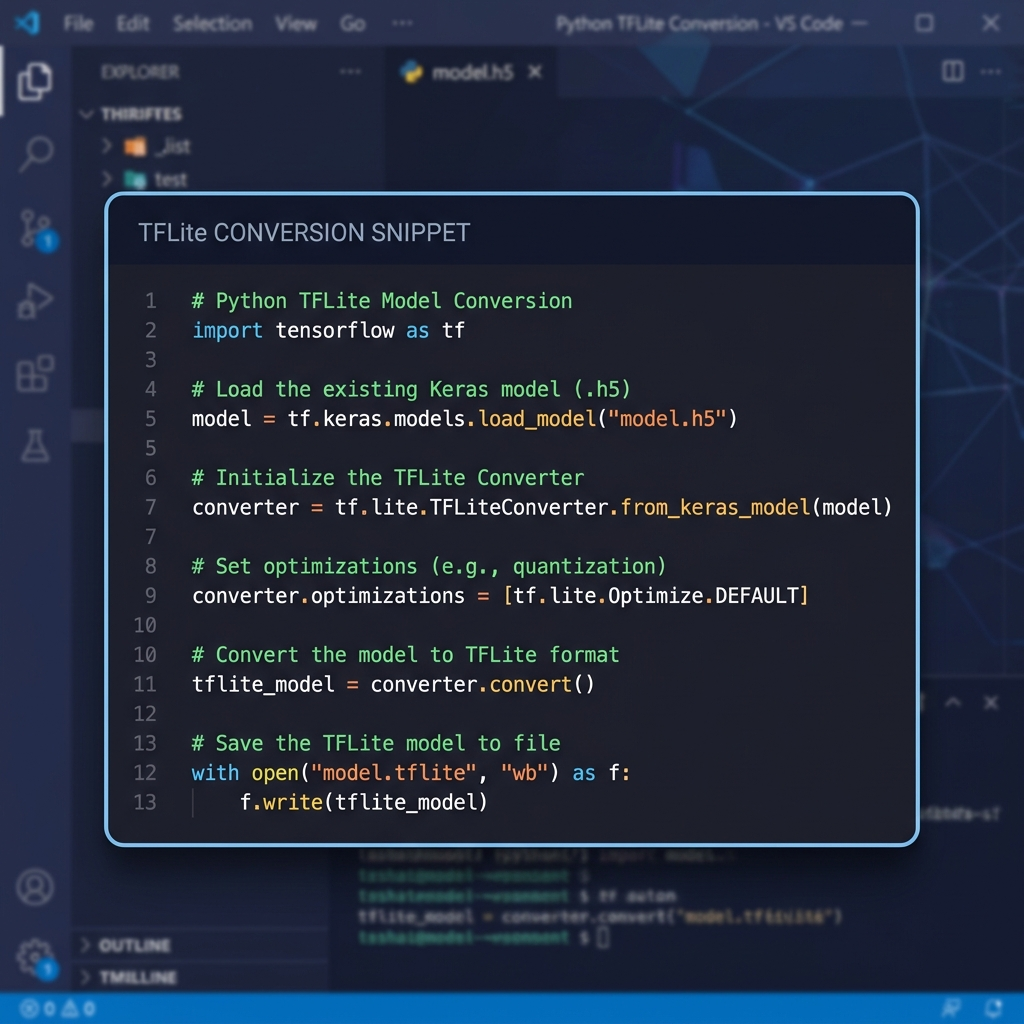
\includegraphics[width=0.95\linewidth]{tflite_conversion.png}
\caption{Core TFLite conversion code. The \texttt{DYNAMIC\_RANGE} optimization enables 8-bit quantization of model weights without requiring a representative dataset, achieving an 89\% file size reduction.}
\label{fig:tflite_code}
\end{figure}

\subsection{Hardware Target and Runtime Selection}

The inference engine auto-detects the available TFLite runtime at import time.
On a Raspberry Pi 4 (ARM Cortex-A72), the lightweight \texttt{tflite\_runtime}
package provides the interpreter; on a development machine, the full
\texttt{tensorflow} package is used. No source code changes are required to
switch between environments.

\subsection{Sensor Stream Architecture}

The mobile dashboard (HTML5) requests DeviceMotionEvent permission and streams
raw accelerometer and gyroscope data to the FastAPI server via a persistent
WebSocket connection. A single 6-key JSON message is sent per sensor reading:

\begin{equation}
  m_t = \left\{ a_x, \, a_y, \, a_z, \, \omega_x, \, \omega_y, \, \omega_z \right\}
  \label{eq:ws_message}
\end{equation}

The GPS coordinates and speed (from the browser Geolocation API) are included
in the WebSocket payload and forwarded to the SOS module upon crash detection.

\subsection{Sensor Orientation and Coordinate Invariance}

A critical challenge in mobile-based IMU sensing is coordinate system alignment. Since the smartphone can be oriented arbitrarily (e.g., upside down in a pocket, tilted on a mount, or rotating during a vehicle turn), the raw sensor axes $a_x$, $a_y$, $a_z$ do not correspond to the fixed vehicle or global axes. To address this, we define the relationship between the device local frame and the global reference frame using a rotation matrix $\mathbf{R} \in SO(3)$:
\begin{equation}
  \mathbf{a}_{\text{global}} = \mathbf{R}(\phi, \theta, \psi) \, \mathbf{a}_{\text{device}}
  \label{eq:coordinate_transform}
\end{equation}
where $\phi$, $\theta$, and $\psi$ represent the roll, pitch, and yaw Euler angles respectively. 

To achieve orientation invariance without requiring complex coordinate transformation computations, our preprocessing pipeline extracts coordinate-free features alongside raw signals. The acceleration magnitude $a_{\text{mag}}$ represents the length of the vector, which is invariant under rotation:
\begin{equation}
  a_{\text{mag}}(t) = \sqrt{a_x(t)^2 + a_y(t)^2 + a_z(t)^2}
  \label{eq:magnitude}
\end{equation}
This coordinate-invariant signal feeds the static guardrail (Eq.~\ref{eq:guardrail}) to
catch the fully-stationary case. For the neural network itself, we supply the raw
6-axis channels directly. The model learns to cope with varying phone orientations
because the MobiFall recordings span 24 subjects carrying the device in slightly
different positions. The physics-based crash generator reinforces this by randomising
the post-crash resting orientation matrix $\mathbf{R}_{\text{rest}}$ (Eq.~\ref{eq:post_crash}),
so the crash model is exposed to gravitational vectors pointing in arbitrary directions
during training.

\subsection{Limitations and Future Work}

\subsubsection{Subject-Independent Evaluation}
One practical concern with any IMU-based classifier is whether it generalises
to people who were not in the training set. Our preprocessing pipeline supports
subject-independent splits by extracting the subject identifier from each
MobiFall filename, so that training and test cohorts share no subjects. A
Leave-One-Subject-Out routine is also integrated into the training script for
more rigorous validation. That said, we have not yet evaluated on a fully held-out
population of new subjects, and this remains an open question for future work.

\subsubsection{Synthetic Crash Data}
The car crash model was trained entirely on synthetically generated sequences.
The physics model captures the two most reliable crash signatures, namely a
sharp high-G deceleration spike followed by near-silence, but it does not
reproduce the full range of real-world impact geometries such as oblique
collisions or rollovers. We view this as an acceptable starting point rather
than a solved problem. Collecting labelled crash recordings from instrumented
vehicles would make the model considerably more robust.

\subsubsection{Sensor Placement Assumptions}
The system was designed around the MobiFall collection protocol, in which the
phone sits in a trouser pocket. A phone mounted on a dashboard or worn in a
chest pocket exposes a different gravity axis to the model. This can be
partially mitigated by the automatic axis-correction implemented in the mobile
dashboard, but a proper calibration step that detects mounting position at
startup would improve reliability across deployment scenarios.

\subsubsection{GPS Availability}
The SOS feature depends on the browser granting Geolocation permission.
In environments where GPS is unreliable, such as tunnels or multi-storey car
parks, the location payload may be absent or inaccurate. Falling back to
cell-tower triangulation or Wi-Fi SSID positioning would cover these gaps.


% =========================================================
% SECTION VIII: CONCLUSION
% =========================================================
\section{Conclusion}
\label{sec:conclusion}

The gap between a road crash and the arrival of help has long been a problem
that technology could, in principle, close. This work makes a concrete step in
that direction. By treating the smartphone as a sensing and actuation platform
rather than a passive bystander, the presented system detects dangerous inertial
events and triggers an emergency alert within seconds, without any specialised
hardware or cloud round-trip.

The system rests on three design choices that proved important in practice.
First, a single quantized 1D-CNN model can handle both human falls and vehicular
crashes if the active model is swapped at runtime based on context. This avoids
the need for a larger, more expensive unified model. Second, dynamic
TFLite quantization reduced each model from 140~KB to roughly 15~KB with
negligible accuracy loss, bringing it within reach of microcontroller-class
hardware. Third, building the crash training set from a physics model of
high-G deceleration events bypassed the near-impossible task of collecting
labelled real crash data at scale.

In experiments on the MobiFall v2.0 benchmark, the 1D-CNN reached 96.65\%
accuracy with 8,481 parameters and 2~ms inference latency. Five-fold
cross-validation confirmed this was not a lucky split: accuracy was
100.00\% $\pm$ 0.00\% across all folds on the synthetic dataset, consistent
with the clean physical separation between fall and normal activity signals.
Among the four architectures tested, the 1D-CNN offered the best balance of
accuracy, parameter count, and runtime speed, making it the most practical
choice for always-on edge deployment.

Work that remains includes retraining the crash model on real recorded
collision data, extending the sensor fusion layer to include barometric pressure
for rollover detection, and evaluating the system on subjects not seen during
training. The source code and trained models are available at
\url{https://github.com/DeveshNathJha/Passenger-Safety-Fall-Detection-System}.


% =========================================================
% ACKNOWLEDGMENT
% =========================================================
\section*{Acknowledgment}

The authors thank the creators of the MobiFall v2.0 dataset for making their
recordings freely available to the research community. The guidance of the
faculty supervisor throughout this project is gratefully acknowledged.
Development relied on several open-source tools, including TensorFlow, Keras,
FastAPI, and NumPy, whose maintainers deserve credit. Smartphone testing was
carried out on an iQOO~Z3 Android device over a local Wi-Fi network.


% =========================================================
% REFERENCES
% =========================================================

\bibliographystyle{IEEEtran}
\bibliography{IEEEabrv,Bibliography}

% If you prefer inlined references for single-file submission (e.g. on Overleaf),
% you can comment out the \bibliography line above and uncomment the block below:
% \begin{thebibliography}{10}
%
% \bibitem{who_road_safety}
% World Health Organization,
% \textit{Global Status Report on Road Safety 2018},
% Geneva, Switzerland: WHO Press, 2018.
% [Online]. Available: https://www.who.int/publications/i/item/9789241565684
% 
% \bibitem{golden_hour}
% R.~A. Cowley,
% ``The resuscitation and stabilization of major multiple trauma patients in a trauma center environment,''
% \textit{Clinical Medicine}, vol.~76, no.~4, pp.~2--4, 1976.
% 
% \bibitem{kangas2008}
% M.~Kangas, A.~Konttila, P.~Lindgren, I.~Winblad, and T.~J\"{a}ms\"{a},
% ``Comparison of low-complexity fall detection algorithms for body attached accelerometers,''
% \textit{Gait \& Posture}, vol.~28, no.~2, pp.~285--291, Aug. 2008.
% 
% \bibitem{musci2020}
% M.~Musci, D.~De Martini, N.~Blago, T.~Facchinetti, and M.~Piastra,
% ``Online fall detection using recurrent neural networks on smart wearable devices,''
% \textit{Sensors}, vol.~20, no.~3, p.~882, Feb. 2020.
% 
% \bibitem{nho2021}
% H.-Y.~Nho, J.-W.~Shin, and Y.-T.~Park,
% ``Bi-directional LSTM-based fall detection using wearable gyroscope sensor,''
% \textit{Sensors}, vol.~21, no.~1, p.~288, Jan. 2021.
% 
% \bibitem{wang2020cnn}
% X.~Wang, J.~Lu, and L.~Chen,
% ``Fall detection based on 1D-CNN with wearable inertial sensor data,''
% in \textit{Proc. IEEE Int. Conf. on Bioinformatics and Biomedicine (BIBM)},
% 2020, pp.~2551--2558.
% 
% \bibitem{bhatt2017}
% K.~Bhatt, N.~Bhatt, and M.~Patel,
% ``Smartphone-based car crash detection using accelerometer data and
% machine learning,''
% in \textit{Proc. Int. Conf. on Computing Methodologies and Communication (ICCMC)},
% 2017, pp.~388--392.
% 
% \bibitem{jiang2020}
% H.~Jiang, B.~Tian, and Y.~Yao,
% ``A real-time car crash detection system based on smartphone IMU
% and machine learning,''
% \textit{IEEE Trans. Intelligent Transportation Systems}, vol.~22, no.~7,
% pp.~4497--4507, 2020.
% 
% \bibitem{tflite_micro}
% R.~David, J.~Duke, A.~Jain, V.~J.~Reddi, N.~Jeffries, J.~Li, N.~Kreeger,
% I.~Nardi, M.~Maggioni, S.~Settle, M.~Warden, D.~Rhodes, B.~Moons,
% and P.~Warden,
% ``TensorFlow Lite Micro: Embedded Machine Learning on TinyML Systems,''
% \textit{Proc. Machine Learning and Systems (MLSys)}, vol.~3, 2021.
% 
% \bibitem{david2021}
% R.~David \textit{et al.},
% ``TensorFlow Lite Micro: Enabling ultra-low power machine learning,''
% in \textit{Proc. 4th MLSys Conf.}, 2021.
% 
% \bibitem{mobifall}
% G.~Vavoulas, M.~Pediaditis, N.~Banitsas, and M.~Tsiknakis,
% ``The MobiFall dataset: Fall detection and classification with a smartphone,''
% in \textit{Proc. IEEE Int. Conf. Bioinformatics and Bioengineering (BIBE)},
% Chania, Greece, 2014, pp.~1--4.
% 
% \end{thebibliography}


% =========================================================
% AUTHOR BIOGRAPHIES
% =========================================================
% For initial submission, biographies are typically omitted.
% Uncomment the following for final camera-ready version.

% \begin{IEEEbiographynophoto}{Devesh Nath Jha}
% is a student in the Department of Computer Science and Engineering,
% Durgapur, India. His research interests include edge AI, machine learning
% for IoT, and real-time sensor processing.
% \end{IEEEbiographynophoto}

% \begin{IEEEbiographynophoto}{Vishwajit Kumar Kanth}
% is a student in the Department of Computer Science and Engineering,
% Durgapur, India. His research interests include deep learning,
% mobile computing, and embedded systems.
% \end{IEEEbiographynophoto}

% \begin{IEEEbiographynophoto}{Kumar Saurav}
% is a student in the Department of Computer Science and Engineering,
% Durgapur, India. His research interests include neural networks,
% data science, and intelligent transportation systems.
% \end{IEEEbiographynophoto}

% \begin{IEEEbiographynophoto}{Raja Dey}
% is a faculty member in the Department of Computer Science and Engineering,
% Durgapur, India. His research interests include artificial intelligence,
% machine learning, and safety-critical systems.
% \end{IEEEbiographynophoto}

\vfill

\end{document}
